\documentclass[11pt,a4paper]{article}

\usepackage[margin=1in]{geometry}
\usepackage{amsmath,amssymb}
\usepackage{booktabs}
\usepackage{enumitem}
%\usepackage[T1]{fontenc}
\usepackage{hyperref}

\usepackage{tikz}     
\usetikzlibrary{positioning, arrows.meta, fit}

\definecolor{boxfill}{HTML}{EAF2FB}
\definecolor{boxdraw}{HTML}{3B6EA8}
\definecolor{hlfill}{HTML}{FDE6D8}
\definecolor{hldraw}{HTML}{D9622B}
\definecolor{subtxt}{HTML}{555555}
\definecolor{plantdraw}{HTML}{6B6B6B}
\definecolor{windfill}{HTML}{E6F4EA}
\definecolor{winddraw}{HTML}{3C8D5A}
% Model and controller names: change them here only.
\newcommand{\KRes}{\textsf{K-Res}}            % Koopman Residual Model (LQR tracking-error dynamics)
\newcommand{\KFull}{\textsf{K-Full}}          % Koopman Full Model (whole outer loop)
\newcommand{\KResMPC}{\textsf{K-Res-MPC}}     % MPC correction on top of the LQR (paper's K-MPC)
\newcommand{\KFullMPC}{\textsf{K-Full-MPC}}   % MPC replacing the LQR
\newcommand{\diag}{\operatorname{diag}}

\title{Koopman MPC for Quadrotor in Turbulent Wind}
\author{Course Project}
\date{\today}



\begin{document}
	\maketitle
	
	\section{Introduction}
	
	\section{Quadrotor Model}
	Usually the quadrotor operating in wind is model with 6 DoF equations shown in Eq. \ref{eqn:quad-wind-model}
	
	\begin{align}
		\dot{p} &= v \\
		\dot{v} &= g e_3 + \frac{1}{m} (R(q) f_T - f_D) \\
		\dot{q} &= \frac{1}{2} q \otimes  \begin{bmatrix}0 \\ \omega \end{bmatrix} \\
		J \dot{\omega} &= \tau_T - \omega \times J \omega 
		\label{eqn:quad-wind-model}
	\end{align}
	
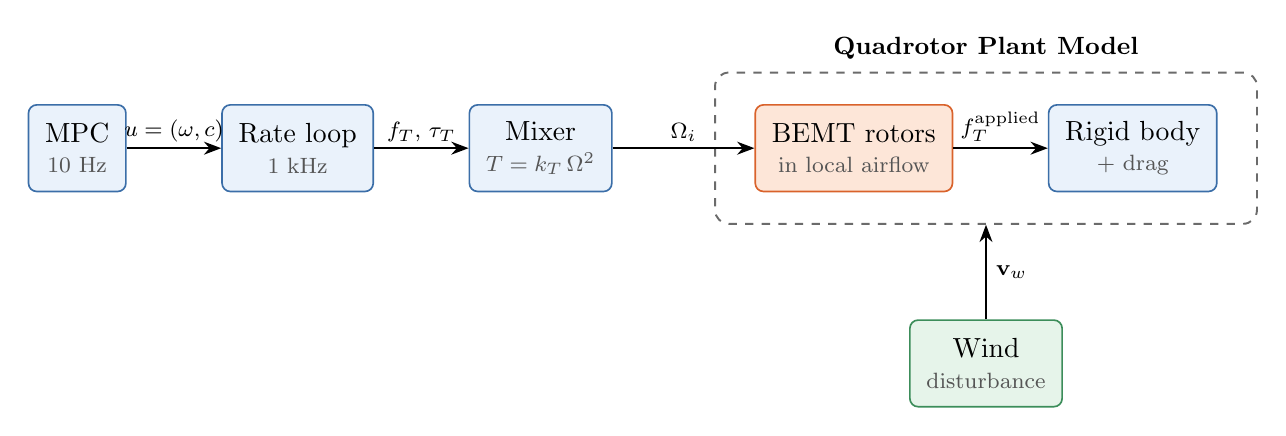
\begin{tikzpicture}[
	node distance = 12mm,
	block/.style = {draw=boxdraw, fill=boxfill, rounded corners=3pt,
		line width=0.6pt, align=center,
		minimum height=11mm, inner xsep=6pt},
	hl/.style    = {block, draw=hldraw, fill=hlfill},
	windb/.style = {block, draw=winddraw, fill=windfill},
	plant/.style = {draw=plantdraw, dashed, rounded corners=5pt,
		line width=0.7pt, inner xsep=5mm, inner ysep=4mm},
	sig/.style   = {-{Stealth[length=2.2mm]}, line width=0.6pt},
	lab/.style   = {above, font=\footnotesize, inner sep=2pt}
	]
	
	% Controller chain
	\node[block] (mpc)  {MPC\\[-1pt] {\footnotesize\color{subtxt}10 Hz}};
	\node[block, right=of mpc]  (rate) {Rate loop\\[-1pt] {\footnotesize\color{subtxt}1 kHz}};
	\node[block, right=of rate] (mix)  {Mixer\\[-1pt] {\footnotesize\color{subtxt}$T = k_T\,\Omega^2$}};
	
	% Plant blocks (extra gap so the input arrow is visible inside the box)
	\node[hl,    right=18mm of mix] (bemt) {BEMT rotors\\[-1pt] {\footnotesize\color{subtxt}in local airflow}};
	\node[block, right=of bemt]     (body) {Rigid body\\[-1pt] {\footnotesize\color{subtxt}+ drag}};
	
	% Plant enclosure
	\node[plant, fit=(bemt)(body)] (plantbox) {};
	\node[above=1pt of plantbox.north, font=\small\bfseries] {Quadrotor Plant Model};
	
	% Wind disturbance
	\node[windb, below=12mm of plantbox] (wind) {Wind\\[-1pt] {\footnotesize\color{subtxt}disturbance}};
	
	% Signals
	\draw[sig] (mpc)  -- node[lab] {$u=(\omega,c)$}         (rate);
	\draw[sig] (rate) -- node[lab] {$f_T,\,\tau_T$}         (mix);
	\draw[sig] (mix)  -- node[lab] {$\Omega_i$}             (bemt);
	\draw[sig] (bemt) -- node[lab] {$f_T^{\text{applied}}$} (body);
	\draw[sig] (wind) -- node[right, font=\footnotesize] {$\mathbf{v}_w$} (plantbox.south);
	
\end{tikzpicture}
	
	\subsection{Blade Element Momentum Theory}
	
	Usually the thrust generated by the rotors are modeled as function of  the rotor angular speed $\Omega_i$ as shown in Eq. \ref{eqn:thrust-model}
	
	\begin{equation}
		\label{eqn:thrust-model}
		T_i = k_f \Omega_i^2
	\end{equation}
	
	In the presence of external wind distrubances, the thrush generated may not exactly follow Eq. \ref{eqn:thrust-model}. Here $k_f$ is an experimentally identified coefficient and it may not be the same for all operating conditions, thus the functional form of thrust is given by Eq. \ref{eqn:generated-thrust}
	
	\begin{equation}
		T_i = f(\Omega_i, V_{\infty}, v_i)
		\label{eqn:generated-thrust}
	\end{equation}
	
	\subsubsection{How is this effect modelled in simulation?}
	
	Blade Element Theory - For a given induced velocity ($v_i$) it calculates the airflow experienced by each rotor blade element which is then integrate to find the lift, drag, and thrust produced by the rotor
	
	\begin{equation}
		T_i = f_{BET}(\Omega, V_{infty}, v_i)
	\end{equation}
	
	Momentum Theory - Instead of examining individual blade elements, it considers the entire rotor as a disk and using conservation of mass and momentum, it finds for a given thrust, what is the induced velocity
	
	\begin{equation}
		T_i = 2 \rho A (V_{infty} + v_i)
	\end{equation}
	
	Both BET and MT equations are solved together to find $v_i and T_i$, since for BET $v_i$  is the input and $T_i$ is the output and it is reversed for MT. Thus both equations are solved simulataneously to obtain the thrust--- which is called as Blade Element Momentum Theory.
		
	\begin{equation}
		f_{BET}(\Omega, V_{infty}, v_i) -  2 \rho A (V_{infty} + v_i) = 0
	\end{equation}
	
	
	\section{Koopman based Quadrotor Modelling}
	\label{sec:koopman}

	\subsection{Koopman operator with inputs}
	For a discrete-time system $x_{k+1} = F(x_k, u_k)$, the Koopman operator acts on observables
	$\psi(x)$ rather than on the state. EDMD approximates it on a finite dictionary
	$\psi = (\psi_1, \dots, \psi_N)$, so that the nonlinear map becomes linear in the lifted state
	$z = \psi(x)$:
	\begin{equation}
		\psi(x_{k+1}) \approx A\,\psi(x_k) + B\,u_k + D\,w_k,
		\qquad \hat{x}_k = C\,z_k,
		\label{eqn:koopman-generic}
	\end{equation}
	where $w_k$ is a measured disturbance (here the wind). The approximation is exact only if
	$\mathrm{span}\{\psi_j\}$ is invariant under the dynamics; otherwise the residual of
	Eq.~\ref{eqn:koopman-generic} is the closure error of the dictionary. In prediction the
	state is lifted once, $z_0 = \psi(x_0)$, and Eq.~\ref{eqn:koopman-generic} is iterated
	without re-lifting, so the MPC sees a linear model and solves a convex QP.

	Two Koopman models are built in this work. They differ in \emph{which system} is identified:
	\begin{itemize}[leftmargin=*]
		\item \textbf{\KRes{}, the Koopman Residual Model}\footnote{``Residual'' here means the
			tracking error left by the LQR. It is the paper's Model~1, not its Model~2, which uses
			the residual \emph{thrust} $f_{\text{res}} = f_c - f_r$.}: the tracking-error dynamics of
			the vehicle \emph{with the LQR in the loop}, driven by a small corrective input. It is
			used by \KResMPC{}, the paper's K-MPC.
		\item \textbf{\KFull{}, the Koopman Full Model}: the dynamics of the vehicle's whole outer
			loop, from the total command $u = (\omega, c)$ to the vehicle state, with no LQR. It is
			used by \KFullMPC{}, which replaces the LQR.
	\end{itemize}
	Naming: a superscript or subscript ${}^{r}$ marks \KRes{} quantities ($\psi_r$, $A_r$,
	$z^r$, \dots) and ${}^{f}$ marks \KFull{} quantities. Table~\ref{tab:koopman-models}
	summarises both.

	\begin{table}[ht]
		\centering
		\caption{The two Koopman models.}
		\label{tab:koopman-models}
		\small
		\begin{tabular}{@{}lll@{}}
			\toprule
			& \KRes{} (Residual) & \KFull{} (Full) \\
			\midrule
			System identified & vehicle + LQR, tracking error & vehicle + rate loop, no LQR \\
			State & $e = x - x_{\text{ref}} \in \mathbb{R}^9$ & $s = [p, v, \eta - \eta^\star, \omega] \in \mathbb{R}^{12}$ \\
			Input & perturbation $u_d \in \mathbb{R}^4$ & $\delta u = u - u^\star \in \mathbb{R}^4$ \\
			Disturbance & $v_w$ & $\delta v_w = v_w - \bar{v}_w$ \\
			Dictionary & monomials, degree $\le 2$ & selective trig.\ monomials, degree $\le 2$ \\
			Lifted dimension $N$ & 55 & 61 \\
			Fit & $\ell_1$-EDMD, $\lambda = 20$ & least squares, translation invariant \\
			Data & 8 episodes, 1112 pairs & 36 episodes, 5004 pairs \\
			Rotor model in data & ideal & BEMT \\
			Controller & \KResMPC{} (on top of LQR) & \KFullMPC{} (replaces LQR) \\
			\bottomrule
		\end{tabular}
	\end{table}

	% ------------------------------------------------------------------------------
	\subsection{\KRes: Koopman Residual Model}
	\label{sec:kres}

	\paragraph{What is learned.}
	A state-dependent LQR (100~Hz) tracks the reference and produces $u_h$. The MPC adds a
	bounded correction $u_d$, so the rate loop receives $u_h + u_d$. Seen from the MPC, the plant
	is the vehicle \emph{together with} the LQR, and the quantity to regulate is the tracking error
	\begin{equation}
		e = \begin{bmatrix} p - p_{\text{ref}} \\ v - v_{\text{ref}} \\ \eta - \eta_{\text{ref}} \end{bmatrix} \in \mathbb{R}^9,
	\end{equation}
	with $\eta = (\phi, \theta, \psi)$ the ZYX Euler angles and the attitude error wrapped to
	$[-\pi, \pi)$. \KRes{} approximates the closed-loop error map
	\begin{equation}
		e_{k+1} = F_r\bigl(e_k,\, u_{d,k},\, v_{w,k}\bigr),
		\label{eqn:kres-true}
	\end{equation}
	which implicitly contains the rigid body, the drag, the rate loop and the LQR gains. Writing it
	as a function of $e$ alone assumes that the error dynamics do not depend on where on the
	reference the vehicle is, which holds only approximately for a state-dependent LQR.

	\paragraph{Model.}
	The error is standardised with the training statistics, $\bar{e} = (e - \mu)\oslash\sigma$, and lifted with all monomials up to degree two:
	\begin{equation}
		\psi_r(\bar{e}) = \bigl(\bar{e}_1, \dots, \bar{e}_9,\; 1,\; \bar{e}_1^2, \bar{e}_1\bar{e}_2, \dots, \bar{e}_9^2\bigr) \in \mathbb{R}^{55},
		\qquad 9 + 1 + 45 = 55.
	\end{equation}
	The \KRes{} model is (paper Eq.~(5))
	\begin{equation}
		\boxed{\;
			z^r_{k+1} = A_r z^r_k + B_r u_{d,k} + D_r v_{w,k}, \qquad
			z^r_0 = \psi_r(\bar{e}_0), \qquad
			\hat{e}_k = \mu + \sigma \odot (C_r z^r_k),
			\;}
		\label{eqn:kres}
	\end{equation}
	with $A_r \in \mathbb{R}^{55\times55}$, $B_r \in \mathbb{R}^{55\times4}$,
	$D_r \in \mathbb{R}^{55\times3}$ and $C_r = [I_9\;\; 0]$. Because the state is the first block of
	$\psi_r$, $C_r$ only selects it. In \KResMPC{} the turbulence is not known ahead of time, so
	the prediction uses $D_r \bar{v}_w$.

	\paragraph{What the approximated model looks like.}
	Projecting one step of Eq.~\ref{eqn:kres} onto the error gives
	\begin{equation}
		\bar{e}_{k+1} = C_r A_r \psi_r(\bar{e}_k) + C_r B_r u_{d,k} + C_r D_r v_{w,k}
		= a_0 + \sum_{i} a_i \bar{e}_{i,k} + \sum_{i \le j} a_{ij} \bar{e}_{i,k}\bar{e}_{j,k} + C_r B_r u_{d,k} + C_r D_r v_{w,k}.
	\end{equation}
	One step is therefore a \emph{quadratic polynomial} of the error with input and wind entering
	linearly. Over several steps the quadratic features are not re-evaluated: they evolve by
	their own rows of $A_r$, which is where the closure error accumulates.

	\paragraph{Training data.}
	The LQR flies two references, a figure-8 ($A, B, C = 3, 1.5, 1$~m, 7~s period) and a circle
	($r = 2$~m, $\pm 0.5$~m vertical, 7~s period), in the Gaussian wind of the paper. The
	perturbation is drawn uniformly, $u_d \sim \mathcal{U}(\pm[0.3, 0.3, 0.3, 1.0])$
	(rad/s, rad/s, rad/s, m/s$^2$), and held for 0.1~s. Four repeats per reference give
	8 training episodes of 14~s at 10~Hz (1112 snapshot pairs), plus one validation repeat per reference.
	Because $u_d$ is drawn independently of the state, it is exogenous to the closed loop.
	This data set was generated with ideal rotors, before the BEMT rotor model was added.

	\paragraph{Fit.}
	With $\Gamma_1 = [\psi_r(\bar{e}_k);\, u_{d,k};\, v_{w,k}]_k$ and
	$\Gamma_2 = [\psi_r(\bar{e}_{k+1})]_k$, $\ell_1$-EDMD (paper Eq.~(8)) solves
	\begin{equation}
		\min_{[A_r\, B_r\, D_r]} \bigl\| \Gamma_2 - [A_r\; B_r\; D_r]\,\Gamma_1 \bigr\|_F^2 + \lambda \bigl\| [A_r\; B_r\; D_r] \bigr\|_1,
		\qquad \lambda = 20,
	\end{equation}
	by coordinate descent. The row of the constant feature is fixed to $e_c^\top$ (it must stay 1),
	so the penalty cannot make it decay over the horizon. The regressor has full rank,
	$62/62$, with condition number $67$.

	% ------------------------------------------------------------------------------
	\subsection{\KFull: Koopman Full Model}
	\label{sec:kfull}

	\paragraph{What is learned.}
	With the LQR removed, the MPC sends the total command to the rate loop: body rates and
	collective thrust, $u = (\omega_x, \omega_y, \omega_z, c)$. The model must then describe the
	open-loop, marginally unstable vehicle.
	\KFull{} approximates
	\begin{equation}
		x_{k+1} = F_f\bigl(x_k,\, u_k,\, v_{w,k}\bigr), \qquad x = (p, v, \eta, \omega) \in \mathbb{R}^{12},
		\label{eqn:kfull-true}
	\end{equation}
	which contains everything between the command and the motion: rigid body, gravity, the thrust
	direction $R(\eta)e_3$, body drag, the rate-loop lag and the BEMT rotor thrust in the local airflow.
	None of the physics-based MPCs in this work model the last two.

	\paragraph{Coordinates.}
	Deviations are taken from the nominal hover trim $x^\star$, $u^\star = (0, 0, 0, g)$, the same
	operating point the nominal LTV MPC uses, so neither model has more prior information.
	The state is scaled but not shifted:
	\begin{equation}
		s = \bigl[p,\; v,\; \eta - \eta^\star,\; \omega\bigr] \oslash \sigma \in \mathbb{R}^{12},
		\qquad \delta u = u - u^\star, \qquad \delta v_w = v_w - \bar{v}_w .
	\end{equation}
	Without a shift, $s = 0$ at the trim, so the origin of the model is the physical equilibrium.
	The body rates are included because gyros measure them and they let the model represent the
	rate-loop lag. They are not penalised in the MPC cost.

	\paragraph{Observables.}
	Position stays linear (translation invariance) and so do the body rates. The nonlinear part of
	the dictionary is built from the velocity and from sines and cosines of the attitude:
	\begin{equation}
		b = \bigl(v_x, v_y, v_z,\; \sin\phi, \cos\phi - 1,\; \sin\theta, \cos\theta - 1,\; \sin\psi, \cos\psi - 1\bigr) \in \mathbb{R}^{9},
	\end{equation}
	\begin{equation}
		\psi_f(s) = \bigl(\,\underbrace{s}_{12},\; \underbrace{1}_{1},\; \underbrace{\sin a, \cos a - 1}_{6,\; a \in \{\phi,\theta,\psi\}},\; \underbrace{b_i b_j,\ i \le j}_{42}\,\bigr) \in \mathbb{R}^{61}.
	\end{equation}
	The degree-two block has 45 products of $b$ minus the three $(\cos a - 1)^2$ terms (see below),
	giving 42.

	\emph{Why trigonometric features of roll and pitch.} The thrust direction is
	\begin{equation}
		R(\eta)e_3 = \begin{bmatrix} c_\psi s_\theta c_\phi + s_\psi s_\phi \\ s_\psi s_\theta c_\phi - c_\psi s_\phi \\ c_\theta c_\phi \end{bmatrix},
	\end{equation}
	so the horizontal force is proportional to $\sin\theta$ and $\sin\phi$, and the vertical one to
	$c\cos\phi\cos\theta$. The latter contains the lift lost to tilt, $c(1 - \cos\theta)$, which the
	hover linearisation drops. The body-frame airspeed $R^\top(v - v_w)$, which sets the drag and
	the rotor inflow (advance ratio $\mu$ and inflow $\lambda_c$ in BEMT), is a sum of
	\emph{velocity $\times$ sin/cos} products. These are exactly the degree-two terms of $b$.
	Polynomials $\phi^2$, $\theta v_x$ approximate the same functions only near level flight.
	Three choices keep the regressor well conditioned:
	\begin{itemize}[leftmargin=*]
		\item $\cos a - 1$ instead of $\cos a$: near hover $\cos a \approx 1$ would duplicate the constant;
		\item $(\cos a - 1)^2$ is omitted, because
		$\sin^2 a + (\cos a - 1)^2 = -2(\cos a - 1)$ is an exact linear dependence;
		\item the raw angles appear only in the linear block, so $C_f$ still reads them out.
	\end{itemize}

	\paragraph{Model.}
	\begin{equation}
		\boxed{\;
			z^f_{k+1} = A_f z^f_k + B_f\,\delta u_k + D_f\,\delta v_{w,k}, \qquad
			z^f_0 = \psi_f(s_0), \qquad
			\delta\hat{x}_k = C_f z^f_k,
			\;}
		\label{eqn:kfull}
	\end{equation}
	with $A_f \in \mathbb{R}^{61\times61}$, $B_f \in \mathbb{R}^{61\times4}$,
	$D_f \in \mathbb{R}^{61\times3}$ and $C_f = [\diag(\sigma_{1..9})\;\; 0]$, which returns the physical
	deviations of $(p, v, \eta)$. Inputs and wind are kept in physical units, so $B_f$ acts on what
	the MPC commands. In \KFullMPC{} $\delta v_w = 0$ in prediction: the mean wind is in the trim,
	and the turbulence is not predicted.

	\paragraph{What the approximated model looks like.}
	One step of Eq.~\ref{eqn:kfull} for the velocity reads
	\begin{equation}
		\delta v_{k+1} = \underbrace{\textstyle\sum_j a^{v}_j s_{j,k}}_{\text{linear}}
		+ a^{v}_0
		+ \underbrace{\textstyle\sum_a \bigl(\alpha^{v}_a \sin a_k + \beta^{v}_a (\cos a_k - 1)\bigr)}_{\text{thrust direction}}
		+ \underbrace{\textstyle\sum_{i \le j} \gamma^{v}_{ij}\, b_{i,k} b_{j,k}}_{\text{drag, BEMT, tilt}}
		+ B^{v}_f \delta u_k + D^{v}_f \delta v_{w,k},
	\end{equation}
	which is the structure of
	$v_{k+1} = v_k + \Delta t\,\bigl(g e_3 - c R(\eta) e_3 - \tfrac{1}{m}(f_D + \Delta f_{\text{BEMT}})\bigr)$
	with every coefficient learned from data rather than derived. Position obeys
	$p_{k+1} = p_k + (\dots)$ with the coefficient of $p_k$ fixed to one (below).

	\paragraph{Training data.}
	Closed-loop data are needed because an open-loop integrator plant drifts away. The episodes
	are flown by the \emph{nominal} LTV MPC, whose model has no drag and so knows nothing about the
	wind, plus a uniform dither
	$d \sim \mathcal{U}(\pm[0.3, 0.3, 0.3, 1.0])$ redrawn every 0.1~s; the \emph{applied} command
	$u = \mathrm{clip}(u_{\text{MPC}} + d)$ is logged. Without the dither, $u$ would be a function of
	$x$ and the regression would recover only the closed loop. References:
	\begin{itemize}[leftmargin=*]
		\item 30 random sum-of-sines references, 3 sinusoids per axis at 0.07--0.25~Hz, peak tilt
		0.05--0.40~rad, horizontal speed $\le 3.5$~m/s, vertical amplitude $\le 1$~m;
		\item 6 hover episodes starting up to $(\pm1, \pm1, \pm0.5)$~m from the set point.
	\end{itemize}
	In total there are 36 episodes of 14~s at 10~Hz, giving 5004 snapshot pairs, with BEMT rotors in the
	Gaussian wind. Circles and figure-8s are kept out of training and validation, so the closed-loop
	tests use trajectory families the model has not seen.

	\paragraph{Fit.}
	Least squares on all blocks together,
	\begin{equation}
		[A_f\; B_f\; D_f] = \Gamma_2 \begin{bmatrix} \psi_f(S) \\ \Delta U \\ \Delta W \end{bmatrix}^{\dagger},
	\end{equation}
	with two structural constraints. The constant row is fixed to $e_c^\top$. The position columns are
	fixed to $A_f[:, p_i] = e_{p_i}$ (\emph{translation invariance}: position may only feed itself).
	The second constraint was introduced after an earlier data set (circles only, all at 2~m altitude,
	$\sigma_{p_z} = 3$~cm) made $p_z$ nearly collinear with the constant. The unconstrained fit then
	split a bias between them that was correct only at 2~m. It is kept for the current data
	($\sigma_{p_z} = 0.24$~m) because it is physics, not a work-around. The lifted regressor has full
	rank, $68/68$, but its condition number is $7.2\times10^{7}$, much larger than for \KRes.

	% ------------------------------------------------------------------------------
	\subsection{Persistency of excitation: the Hankel matrix test}
	\label{sec:pe}

	For an input sequence $u_1, \dots, u_T$ with $l$ channels, the depth-$L$ block-Hankel matrix is
	\begin{equation}
		H_L(u) = \begin{bmatrix}
			u_1 & u_2 & \cdots & u_{T-L+1} \\
			u_2 & u_3 & \cdots & u_{T-L+2} \\
			\vdots & \vdots & & \vdots \\
			u_L & u_{L+1} & \cdots & u_T
		\end{bmatrix} \in \mathbb{R}^{lL \times (T-L+1)} .
	\end{equation}
	The input is \emph{persistently exciting (PE) of order $L$} if $\operatorname{rank} H_L(u) = lL$,
	which needs at least $T \ge (l+1)L - 1$ samples. By Willems' fundamental lemma, if a
	controllable LTI system with $n$ states is driven by an input that is PE of order $n + 1$, then
	$\operatorname{rank}[X; U] = n + l$, and the regression for $[A\;B]$ has a unique solution. The
	lemma needs controllability, not full actuation, so it applies to the underactuated quadrotor.

	Implementation details:
	\begin{itemize}[leftmargin=*]
		\item Episodes are short, so they are combined in a \emph{mosaic} Hankel matrix
		$[H_L(u^{(1)})\; \cdots\; H_L(u^{(r)})]$, and no window crosses an episode boundary.
		At $L = N + 1$ one episode of 140 samples is below $(l+1)L - 1$, so only the collection of
		episodes can be PE at that order.
		\item The rank uses the relative threshold $\sigma_i/\sigma_{\max} > 10^{-9}$, and
		$\sigma_{\min}/\sigma_{\max}$ is reported, because it shows how close the data are to losing
		excitation.
		\item Orders tested: $n + 1$ (Willems' lemma on the physical state), the same with the wind
		channels appended ($l = 7$), and $N + 1$ (the lifted dimension).
	\end{itemize}

	\begin{table}[ht]
		\centering
		\caption{Hankel test on the training inputs (\texttt{koopman/excitation.py}).
			\KRes{}: $u_d$, data set \texttt{20261107T182512Z\_datagen\_model1}, recorded in run
			\texttt{20261119T152936Z\_edmd\_model1}.
			\KFull{}: $\delta u$, data set \texttt{20261118T192413Z\_outer\_loop\_data}.}
		\label{tab:pe}
		\small
		\begin{tabular}{@{}llrrrc@{}}
			\toprule
			Model & Test & rank / $lL$ & columns & $\sigma_{\min}/\sigma_{\max}$ & PE \\
			\midrule
			\KRes{} ($n = 9$, $N = 55$) & input, $L = n+1 = 10$ & 40 / 40 & 1048 & 0.240 & yes \\
			& input + wind, $L = 10$ & 70 / 70 & 1048 & 0.0066 & yes \\
			& input, $L = N+1 = 56$ & 224 / 224 & 680 & 0.107 & yes \\
			\midrule
			\KFull{} ($n = 12$, $N = 61$) & input, $L = n+1 = 13$ & 52 / 52 & 4608 & 0.055 & yes \\
			& input + wind, $L = 13$ & 91 / 91 & 4608 & 0.026 & yes \\
			& input, $L = N+1 = 62$ & 248 / 248 & 2844 & 0.016 & yes \\
			\bottomrule
		\end{tabular}
	\end{table}

	\paragraph{Reading the results.}
	Both input sets are PE at every order tested (Table~\ref{tab:pe}).
	\begin{itemize}[leftmargin=*]
		\item \KRes{} passes with the larger margin ($\sigma_{\min}/\sigma_{\max} = 0.24$ at $n+1$),
		but partly by construction: $u_d$ is an independent uniform sequence, which is PE of any order
		it has samples for. The test shows that the perturbation excites the LQR closed loop. It
		says nothing about whether the data identify the vehicle itself.
		\item \KFull{} has the harder case: its input is mostly MPC feedback, and only the dither makes
		it PE. The lower margin (0.055) reflects that.
		\item In both models the wind channels are the weakest direction (0.0066 and 0.026). The likely
		cause is the small vertical wind variance (0.0064~(m/s)$^2$), which leaves the vertical-wind
		column of $D$ less well determined.
	\end{itemize}
	The Hankel test is necessary but not sufficient for a lifted model: Willems' lemma is a result for
	linear systems, and EDMD's uniqueness depends on the rank of the lifted regressor
	$[\psi(X); U; W]$, which is reported with each fit above. The altitude problem of \KFull{} is an
	example: both tests passed, yet one direction ($p_z$ against the constant) was poorly determined.
	Known structure, not more rank, fixed it.
	
	\section{Model Predictive Control}
	
	\subsection{MPC as corrective controller}
	
	\subsection{MPC with Quadrotor model identified with Koopman}
	
	\subsection{MPC with linearized Quadrotor model}
	
	\section{Results}
	
	\section{Conclusion}
	
\end{document}